\documentclass[11pt]{article}
\usepackage{float}
\usepackage{fullpage}
\usepackage{amsmath}
\usepackage{amstext}
\usepackage{caption}

\title{Computer Architecture (ECS 154A) Study Guide}
\author{Davis Computer Science Club --- Tutoring Committee}
\date{Winter Quarter 2015}

\usepackage{tikz}
\usetikzlibrary{arrows}
\usetikzlibrary{matrix,calc}

%isolated term
%#1 - Optional. Space between node and grouping line. Default=0
%#2 - node
%#3 - filling color
\newcommand{\implicantsol}[3][0]{
	\draw[rounded corners=3pt, fill=#3, opacity=0.3] ($(#2.north west)+(135:#1)$) rectangle ($(#2.south east)+(-45:#1)$);
}


%internal group
%#1 - Optional. Space between node and grouping line. Default=0
%#2 - top left node
%#3 - bottom right node
%#4 - filling color
\newcommand{\implicant}[4][0]{
	\draw[rounded corners=3pt, fill=#4, opacity=0.3] ($(#2.north west)+(135:#1)$) rectangle ($(#3.south east)+(-45:#1)$);
}

%group lateral borders
%#1 - Optional. Space between node and grouping line. Default=0
%#2 - top left node
%#3 - bottom right node
%#4 - filling color
\newcommand{\implicantcostats}[4][0]{
	\draw[rounded corners=3pt, fill=#4, opacity=0.3] ($(rf.east |- #2.north)+(90:#1)$)-| ($(#2.east)+(0:#1)$) |- ($(rf.east |- #3.south)+(-90:#1)$);
	\draw[rounded corners=3pt, fill=#4, opacity=0.3] ($(cf.west |- #2.north)+(90:#1)$) -| ($(#3.west)+(180:#1)$) |- ($(cf.west |- #3.south)+(-90:#1)$);
}

%group top-bottom borders
%#1 - Optional. Space between node and grouping line. Default=0
%#2 - top left node
%#3 - bottom right node
%#4 - filling color
\newcommand{\implicantdaltbaix}[4][0]{
	\draw[rounded corners=3pt, fill=#4, opacity=0.3] ($(cf.south -| #2.west)+(180:#1)$) |- ($(#2.south)+(-90:#1)$) -| ($(cf.south -| #3.east)+(0:#1)$);
	\draw[rounded corners=3pt, fill=#4, opacity=0.3] ($(rf.north -| #2.west)+(180:#1)$) |- ($(#3.north)+(90:#1)$) -| ($(rf.north -| #3.east)+(0:#1)$);
}

%group corners
%#1 - Optional. Space between node and grouping line. Default=0
%#2 - filling color
\newcommand{\implicantcantons}[2][0]{
	\draw[rounded corners=3pt, opacity=.3] ($(rf.east |- 0.south)+(-90:#1)$) -| ($(0.east |- cf.south)+(0:#1)$);
	\draw[rounded corners=3pt, opacity=.3] ($(rf.east |- 8.north)+(90:#1)$) -| ($(8.east |- rf.north)+(0:#1)$);
	\draw[rounded corners=3pt, opacity=.3] ($(cf.west |- 2.south)+(-90:#1)$) -| ($(2.west |- cf.south)+(180:#1)$);
	\draw[rounded corners=3pt, opacity=.3] ($(cf.west |- 10.north)+(90:#1)$) -| ($(10.west |- rf.north)+(180:#1)$);
	\fill[rounded corners=3pt, fill=#2, opacity=.3] ($(rf.east |- 0.south)+(-90:#1)$) -|  ($(0.east |- cf.south)+(0:#1)$) [sharp corners] ($(rf.east |- 0.south)+(-90:#1)$) |-  ($(0.east |- cf.south)+(0:#1)$) ;
	\fill[rounded corners=3pt, fill=#2, opacity=.3] ($(rf.east |- 8.north)+(90:#1)$) -| ($(8.east |- rf.north)+(0:#1)$) [sharp corners] ($(rf.east |- 8.north)+(90:#1)$) |- ($(8.east |- rf.north)+(0:#1)$) ;
	\fill[rounded corners=3pt, fill=#2, opacity=.3] ($(cf.west |- 2.south)+(-90:#1)$) -| ($(2.west |- cf.south)+(180:#1)$) [sharp corners]($(cf.west |- 2.south)+(-90:#1)$) |- ($(2.west |- cf.south)+(180:#1)$) ;
	\fill[rounded corners=3pt, fill=#2, opacity=.3] ($(cf.west |- 10.north)+(90:#1)$) -| ($(10.west |- rf.north)+(180:#1)$) [sharp corners] ($(cf.west |- 10.north)+(90:#1)$) |- ($(10.west |- rf.north)+(180:#1)$) ;
}

%Empty Karnaugh map 4x4
\newenvironment{Karnaugh}%
{
	\begin{tikzpicture}[baseline=(current bounding box.north),scale=0.8]
	\draw (0,0) grid (4,4);
	\draw (0,4) -- node [pos=1,above right,anchor=south west] {\( x_1 x_0 \)} node [pos=0.7,below left,anchor=north east] {\( x_3 x_2\)} ++(135:1);
	%
	\matrix (mapa) [matrix of nodes,
	column sep={0.8cm,between origins},
	row sep={0.8cm,between origins},
	every node/.style={minimum size=0.3mm},
	anchor=8.center,
	ampersand replacement=\&] at (0.5,0.5)
	{
		\& |(c00)| 00         \& |(c01)| 01         \& |(c11)| 11         \& |(c10)| 10         \& |(cf)| \phantom{00} \\
		|(r00)| 00             \& |(0)|  \phantom{0} \& |(1)|  \phantom{0} \& |(3)|  \phantom{0} \& |(2)|  \phantom{0} \&                     \\
		|(r01)| 01             \& |(4)|  \phantom{0} \& |(5)|  \phantom{0} \& |(7)|  \phantom{0} \& |(6)|  \phantom{0} \&                     \\
		|(r11)| 11             \& |(12)| \phantom{0} \& |(13)| \phantom{0} \& |(15)| \phantom{0} \& |(14)| \phantom{0} \&                     \\
		|(r10)| 10             \& |(8)|  \phantom{0} \& |(9)|  \phantom{0} \& |(11)| \phantom{0} \& |(10)| \phantom{0} \&                     \\
		|(rf) | \phantom{00}   \&                    \&                    \&                    \&                    \&                     \\
	};
}%
{
	\end{tikzpicture}
}

%Empty Karnaugh map 2x4
\newenvironment{Karnaughvuit}%
{
	\begin{tikzpicture}[baseline=(current bounding box.north),scale=0.8]
	\draw (0,0) grid (4,2);
	\draw (0,2) -- node [pos=1,above right,anchor=south west] {\(x_1 x_0\)} node [pos=0.7,below left,anchor=north east] {\(x_2\)} ++(135:1);
	%
	\matrix (mapa) [matrix of nodes,
	column sep={0.8cm,between origins},
	row sep={0.8cm,between origins},
	every node/.style={minimum size=0.3mm},
	anchor=4.center,
	ampersand replacement=\&] at (0.5,0.5)
	{
		\& |(c00)| 00         \& |(c01)| 01         \& |(c11)| 11         \& |(c10)| 10         \& |(cf)| \phantom{00} \\
		|(r00)| 0             \& |(0)|  \phantom{0} \& |(1)|  \phantom{0} \& |(3)|  \phantom{0} \& |(2)|  \phantom{0} \&                     \\
		|(r01)| 1             \& |(4)|  \phantom{0} \& |(5)|  \phantom{0} \& |(7)|  \phantom{0} \& |(6)|  \phantom{0} \&                     \\
		|(rf) | \phantom{00}  \&                    \&                    \&                    \&                    \&                     \\
	};
}%
{
	\end{tikzpicture}
}

%Empty Karnaugh map 2x2
\newenvironment{Karnaughquatre}%
{
	\begin{tikzpicture}[baseline=(current bounding box.north),scale=0.8]
	\draw (0,0) grid (2,2);
	\draw (0,2) -- node [pos=0.7,above right,anchor=south west] {b} node [pos=0.7,below left,anchor=north east] {a} ++(135:1);
	%
	\matrix (mapa) [matrix of nodes,
	column sep={0.8cm,between origins},
	row sep={0.8cm,between origins},
	every node/.style={minimum size=0.3mm},
	anchor=2.center,
	ampersand replacement=\&] at (0.5,0.5)
	{
		\& |(c00)| 0          \& |(c01)| 1  \\
		|(r00)| 0 \& |(0)|  \phantom{0} \& |(1)|  \phantom{0} \\
		|(r01)| 1 \& |(2)|  \phantom{0} \& |(3)|  \phantom{0} \\
	};
}%
{
	\end{tikzpicture}
}

%Defines 8 or 16 values (0,1,X)
\newcommand{\contingut}[1]{%
	\foreach \x [count=\xi from 0]  in {#1}
	\path (\xi) node {\x};
}

%Places 1 in listed positions
\newcommand{\minterms}[1]{%
	\foreach \x in {#1}
	\path (\x) node {1};
}

%Places 0 in listed positions
\newcommand{\maxterms}[1]{%
	\foreach \x in {#1}
	\path (\x) node {0};
}

%Places X in listed positions
\newcommand{\indeterminats}[1]{%
	\foreach \x in {#1}
	\path (\x) node {X};
}

\begin{document}

\begin{titlepage}
\maketitle
\end{titlepage}

\tableofcontents

\pagebreak

\section{Boolean Algebra}

\subsection{Operations}

\begin{table}[H]
	\centering
	\begin{tabular}{c | c | c}
		Operation	&	Symbol			&	Example\\
		\hline
		NOT			&	\( \bar{ } \)	&	\( \bar{A} \)\\
					&	\( ! \)			&	\( !A \)\\
					&	\( \neg \)		&	\( \neg A \)\\
					&	\( \sim \)		&	\( \sim A \)\\
		\hline
		AND			&	\( \wedge \)	&	\( A \wedge B \)\\
					&	\( * \)			&	\( A * B \)\\
					&					&	\( AB \)\\
		\hline
		OR			&	\( \vee \)		&	\( A \vee B \)\\
					&	\( + \)			&	\( A + B\)\\
		\hline
		XOR			&	\( \oplus \)	&	\( A \oplus B \)
	\end{tabular}
\end{table}

\subsection{Equivalence Laws}

\begin{table}[H]
	\centering
	\begin{tabular}{l | l | l}
		Name			&	OR Version										&	AND Version\\
		\hline
		Commutative		&	\( A + B  = B + A \)							&	\( A * B = B * A \)\\
		Associative		&	\( (A + B) + C = A + (B + C) \)					&	\( (A * B) * C = A * (B * C) \)\\
		Distributive	&	\( A + (B * C) = (A + B) * (A + C) \)			&	\( A * (B + C) = (A * B) + (A * C) \)\\
		Identity		&	\( A + 0 = A \)									&	\( A * 1 = A \)\\
		Annulment		&	\( A + 1 = 1 \)									&	\( A * 0 = 0 \)\\
		Idempotent		&	\( A + A = A \)									&	\( A * A = A \)\\
		Complement		&	\( A + \bar{A} = 1 \)							&	\( A * \bar{A} = 0 \)\\
		De Morgan's		&	\( \overline{(A + B)} = \bar{A} * \bar{B} \)	&	\( \overline{(A * B)} = \bar{A} + \bar{B} \)
	\end{tabular}
\end{table}

\subsection{Truth Table}

Truth tables are mathematical tables composing of every combination of inputs and the resulting function. The number of combinations or rows in the truth table is \( 2^N \), where N is the number of inputs.

\subsubsection{NOT}

\begin{table}[H]
	\centering
	\begin{tabular}{c | c}
		A	&	\( f(A) = !A \)\\
		\hline
		0	&	1\\
		1	&	0
	\end{tabular}
\end{table}

\subsubsection{AND}

\begin{table}[H]
	\centering
	\begin{tabular}{c c | c}
		A	&	B	&	\( f(A,B) = A * B \)\\
		\hline
		0	&	0	&	0\\
		0	&	1	&	0\\
		1	&	0	&	0\\
		1	&	1	&	1
	\end{tabular}
\end{table}

\subsubsection{OR}

\begin{table}[H]
	\centering
	\begin{tabular}{c c | c}
		A	&	B	&	\( f(A,B) = A + B \)\\
		\hline
		0	&	0	&	0\\
		0	&	1	&	1\\
		1	&	0	&	1\\
		1	&	1	&	1
	\end{tabular}
\end{table}

\subsubsection{XOR}

\begin{table}[H]
	\centering
	\begin{tabular}{c c | c}
		A	&	B	&	\( f(A,B) = A \oplus B \)\\
		\hline
		0	&	0	&	0\\
		0	&	1	&	1\\
		1	&	0	&	1\\
		1	&	1	&	0
	\end{tabular}
\end{table}

\subsubsection{Example}

\textbf{Create a function that takes three inputs --- x2, x1, x0 --- and produces a high or on signal when only two input signals are on.}

\begin{table}[H]
	\centering
	\begin{tabular}{c c c | c}
		x2	&	x1	&	x0	&	\( f(x2,x1,x0) \)\\
		\hline
		0	&	0	&	0	&	0\\
		0	&	0	&	1	&	0\\
		0	&	1	&	0	&	0\\
		0	&	1	&	1	&	1\\
		1	&	0	&	0	&	0\\
		1	&	0	&	1	&	1\\
		1	&	1	&	0	&	1\\
		1	&	1	&	1	&	0
	\end{tabular}
\end{table}

\subsection{Canonical Disjunctive Normal Form}

\subsubsection{Minterm}

The canonical disjunctive normal form is also known as a minterm, typically represented by a lower case `m'. A minterm is a logical product term such that it uses each input variable once and it uses only the complement operator and conjunction operation. In other words, if there are n input variables, the minterm must keep to the following constraints: 
\begin{enumerate}
	\item be a logical product that evaluates to logically true
	\item use each of the n variables once
	\item only use NOT operators and AND operators
\end{enumerate}

\noindent For three inputs, the minterms are as follows:

\begin{table}[H]
	\centering
	\begin{tabular}{c c c | c | c}
		\( x_2 \)	&	\( x_1 \)	&	\( x_0 \)	&	&	Minterm (Product Term)\\
		\hline
		0			&	0			&	0		&	\( m_0 \)	&	\( \bar{x_2} \bar{x_1} \bar{x_0} \) \\	
		0			&	0			&	1		&	\( m_1 \)	&	\( \bar{x_2} \bar{x_1} x_0 \) \\
		0			&	1			&	0		&	\( m_2 \)	&	\( \bar{x_2} x_1 \bar{x_0} \) \\
		0			&	1			&	1		&	\( m_3 \)	&	\( \bar{x_2} x_1 x_0 \) \\
		1			&	0			&	0		&	\( m_4 \)	&	\( x_2 \bar{x_1} \bar{x_0} \) \\
		1			&	0			&	1		&	\( m_5 \)	&	\( x_2 \bar{x_1} x_0 \) \\
		1			&	1			&	0		&	\( m_6 \)	&	\( x_2 x_1 \bar{x_0} \) \\
		1			&	1			&	1		&	\( m_7 \)	&	\( x_2 x_1 x_0 \) \\
	\end{tabular}
	\caption*{Note: Product terms all evaluate to be logically true.}
\end{table}

\noindent For a given function, \( f \), it is possible to express the function as a ``sum of products". This is a special form of the canonical normal form in that it only includes terms such that it makes the function logically true.

\subsubsection{Example}

\textbf{Create a function that takes three inputs --- x2, x1, x0 --- and produces a high or on signal when only two input signals are on. Express this function as a sum of products.}

\begin{table}[H]
	\centering
	\begin{tabular}{c c c c | c}
				&	x2	&	x1	&	x0	&	\( f(x2,x1,x0) \)\\
		\hline
					&	0	&	0	&	0	&	0\\
					&	0	&	0	&	1	&	0\\
					&	0	&	1	&	0	&	0\\
		\( m_3 \)	&	0	&	1	&	1	&	1\\
					&	1	&	0	&	0	&	0\\
		\( m_5 \)	&	1	&	0	&	1	&	1\\
		\( m_6 \)	&	1	&	1	&	0	&	1\\
					&	1	&	1	&	1	&	0
	\end{tabular}
\end{table}

\begin{eqnarray*}
	f(x_2,x_1,x_0) &=& m_3 + m_5 + m_6\\
		&=& (\bar{x_2} x_1 x_0) + (x_2 \bar{x_1} x_0) + (x_2 x_1 \bar{x_0})
\end{eqnarray*}

\subsection{Canonical Conjunctive Normal Form}

\subsubsection{Maxterm}

The canonical conjunctive normal form is also known as a maxterm, typically represented by a lower case `M'. A maxterm is a logical sum term such that it uses each input variable once and it uses only the complement operator and disjunction operation. In other words, if there are n input variables, the minterm must keep to the following constraints: 
\begin{enumerate}
	\item be a logical sum that evaluates to logically false
	\item use each of the n variables once
	\item only use NOT operators and OR operators
\end{enumerate}

\noindent For three inputs, the maxterms are as follows:

\begin{table}[H]
	\centering
	\begin{tabular}{c c c | c | c}
		\( x_2 \)	&	\( x_1 \)	&	\( x_0 \)	&	&	Maxterm (Sum Term)\\
		\hline
		0			&	0			&	0		&	\( M_0 \)	&	\( x_2 + x_1 + x_0 \) \\	
		0			&	0			&	1		&	\( M_1 \)	&	\( x_2 + x_1 + \bar{x_0} \) \\
		0			&	1			&	0		&	\( M_2 \)	&	\( x_2 + \bar{x_1} + x_0 \) \\
		0			&	1			&	1		&	\( M_3 \)	&	\( x_2 + \bar{x_1} + \bar{x_0} \) \\
		1			&	0			&	0		&	\( M_4 \)	&	\( \bar{x_2} + x_1 + x_0 \) \\
		1			&	0			&	1		&	\( M_5 \)	&	\( \bar{x_2} + x_1 + \bar{x_0} \) \\
		1			&	1			&	0		&	\( M_6 \)	&	\( \bar{x_2} + \bar{x_1} + x_0 \) \\
		1			&	1			&	1		&	\( M_7 \)	&	\( \bar{x_2} + \bar{x_1} + \bar{x_0} \) \\
	\end{tabular}
	\caption*{Note: Sum terms all evaluate to be logically false.}
\end{table}

\noindent For a given function, \( f \), it is possible to express the function as a ``product of sums". This is a special form of the canonical normal form in that it only includes values such that it makes the function logically false.

\subsubsection{Example}

\textbf{Create a function that takes three inputs --- x2, x1, x0 --- and produces a high or on signal when only two input signals are on. Express this function as a product of sums.}

\begin{table}[H]
	\centering
	\begin{tabular}{c c c c | c}
		&	x2	&	x1	&	x0	&	\( f(x2,x1,x0) \)\\
		\hline
		\( M_0 \)	&	0	&	0	&	0	&	0\\
		\( M_1 \)	&	0	&	0	&	1	&	0\\
		\( M_2 \)	&	0	&	1	&	0	&	0\\
					&	0	&	1	&	1	&	1\\
		\( M_4 \)	&	1	&	0	&	0	&	0\\
					&	1	&	0	&	1	&	1\\
					&	1	&	1	&	0	&	1\\
		\( M_7 \)	&	1	&	1	&	1	&	0
	\end{tabular}
\end{table}

\begin{eqnarray*}
	f(x_2,x_1,x_0) &=& M_0 * M_1 * M_2 * M_4 * M_7\\
		&=& (x_2 + x_1 + x_0) * (x_2 + x_1 + \bar{x_0}) * (x_2 + \bar{x_1} + x_0) * (\bar{x_2} + x_1 + x_0) * (\bar{x_2} + \bar{x_1} + \bar{x_0})
\end{eqnarray*}

\subsection{Karnaugh Maps}

Karnaugh maps are a visual methodology to simplifying boolean expressions. When setting up the Karnaugh map, input values cannot differ more than one hamming distance. The resulting expressions are either a sum of products or a product of sums.

\subsubsection{Example (Three Variables)}

\textbf{Find a minimum sum of products expression for \( f(x_2,x_1,x_0) = m_1 + m_4 + m_5 + m_7 \).}
	
\begin{figure}[H]
	\centering
    \begin{Karnaughvuit}
    	\minterms{1,4,5,7}
    	\maxterms{0,2,3,6}
    	\implicant{1}{5}{green}
    	\implicant{4}{5}{blue}
    	\implicant{5}{7}{red}
    \end{Karnaughvuit}
\end{figure}

\vspace{-1cm}

\[ f(x_2,x_1,x_0) = (\bar{x_1} x_0) + (x_2 \bar{x_1}) + (x_2 x_0) \]

\subsubsection{Example (Four Variables)}

\textbf{Find a minimum product of sums expression for \( f(x_3,x_2,x_1,x_0) = m_0 + m_2 + m_6 + m_8 + m_9 + m_{10} + m_{14} + D_{15} \).}

\begin{figure}[H]
	\centering
    \begin{Karnaugh}
    	\contingut{1,0,1,0,0,0,1,0,1,1,1,0,0,0,1,X}
    	\implicant{3}{11}{red}
    	\implicant{1}{7}{blue}
    	\implicant{4}{13}{green}
    \end{Karnaugh}
\end{figure}

\vspace{-1cm}

\[ f(x_3,x_2,x_1,x_0) = (x_3 + \bar{x_0}) * (\bar{x_2} + x_1) * (\bar{x_1} + \bar{x_0}) \]

\subsubsection{Example (Five Variables)}

\subsection{Quine-McClucksey Algorithm}

\section{Combinational Logic Circuits}

\subsection{Gates}

\subsection{Timing Diagrams}

\subsection{Multiplexers, Decoders, Shifters}

\subsection{Adders and Subtracters}

\subsection{Designing Combinational Logic Circuits}

\section{Finite State Automata}

\subsection{Moore Model}

\subsection{Mealy Model}

\section{Sequential Logic Circuit}

\subsection{Latches}

\subsection{Flip Flops}

\subsection{Registers and Counters}

\subsection{Designing Sequential Logic Circuits}

\section{Single Cycle CPU Design}

\section{Cache}

Effectiveness is based on the concept of information reuse: temporal locality and spatial locality.

\subsection{Memory Hierarchy}

Goal: Make memory perform as if it was made of the most expensive and fastest type, but cost as if made of the cheapest type.

\begin{enumerate}
	\item Fast, Hot, Expensive
	\item Static RAM
	\item Dynamic RAM
	\item Disk
\end{enumerate}

\noindent A cache is smaller than main memory and is composed of numerous cache lines. Cache lines consist of a dirty bit, a tag, and block(s) of data. If the dirty bit is on, then it signals the CPU to write the data from this cache line into main memory when this cache line is freed. Caches also contain a valid bit which signifies whether there is loaded data into the cache --- imagine starting up the computer for the first time, the cache is going to be empty. The issue is that even when a cache is empty (bits are all 0), it still holds some signal. As we continue, when we mention the size of a cache line, we refer to the size of the data blocks in the cache line only (excluding flags and tag).

\begin{table}[H]
	\centering
	\begin{tabular}{| c | c | c |}
		\hline
		Flags	&	\hspace{.5cm} Tag \hspace{.5cm} 		&	\hspace{1cm} Block(s) \hspace{1cm} \\
		\hline
	\end{tabular}
\end{table}

\subsection{Direct Mapped Cache}

A given address is partitioned into three components: Tag, line number, and offset. The line number directly accesses a specific cache line. It then compares the tag partitioned from the address to the tag stored in the cache line. If the tags match, then it is a cache hit. Otherwise, it becomes a cache miss. Assuming that it was a cache hit, it then proceeds to use the offset to select which block to read or write. The block of data in the cache line can be thought of as an array and the offset as an index into this ``array".

\subsubsection{Format}

\begin{table}[H]
	\centering
	\begin{tabular}{| c | c | c |}
		\hline
		Tag		&	Line Number		&		 Offset\\
		\hline
	\end{tabular}
\end{table}

\subsubsection{Example}

\textbf{A CPU is using 24-bit addresses and is byte-addressable. Each line in cache holds 16 bytes of data and each block is 1 byte. Assuming that the tag is 12 bits wide, find the following: number of lines in cache, size of cache, size of tag, and sizes of each partition in the format.}

\[
\text{Size(Cache Line)} = 16 \text{ bytes}
\]
\begin{eqnarray*}
	\text{Bit\_Width(Offset)} &=& \text{Number of bits needed to address 16 blocks}\\
		&=& \log_2 16\\
		&=& 4 \text{ bits}
\end{eqnarray*}
\begin{eqnarray*}
\text{Bit\_Width(Line Number)} &=& \text{Size(Address)} - \text{Bit\_Width(Tag)} - \text{Bit\_Width(Offset)}\\
	&=& 24 \text{ bits} - 12 \text{ bits} - 4 \text{ bits}\\
	&=& 8 \text{ bits}
\end{eqnarray*}
\begin{eqnarray*}
	\text{Number of Cache Lines} &=& 2^\text{Bit\_Width(Line Number)}\\
		&=& 2^8\\
		&=& 256
\end{eqnarray*}
\begin{eqnarray*}
	\text{Size of Cache} &=& \text{Number of Cache Lines} * \text{Size of Cache Lines}\\
		&=& 2^8 * 2^4\\
		&=& 2048 \text{ bytes}\\
		&=& 2 \text{ KB}
\end{eqnarray*}

\begin{table}[H]
	\centering
	\caption*{Format Partition Sizes and Bit Range}
	\begin{tabular}{| c | c | c | c |}
		\hline
					&	Tag		&	Line Number		&	Offset\\
		\hline
		Size		&	12 Bits	&	8 Bits			&	4 Bits\\
		\hline
		Bit Range	&	[12,23]	&	[4,11]	&	[0,3]\\
		\hline
	\end{tabular}
\end{table}

\noindent The bit range represents what bits that partition occupies. Ex: Offset occupies bits 0, 1, 2, and 3. The four least-significant bits.

\subsection{Fully Associative}

A given address is partitioned into two components: Tag and offset. The reason why a line number is unused is because the CPU will perform a linear search through all cache lines looking for either a cache hit, an unused cache line, or a cache line to replace. Because of this, using full association has the lowest miss rates. The tag and offset performs the same as the tag and offset in direct mapping.


\subsubsection{Format}

\begin{table}[H]
	\centering
	\begin{tabular}{| c | c |}
		\hline
		Tag			&		 Offset\\
		\hline
	\end{tabular}
\end{table}

\subsubsection{Example}

\textbf{A CPU is using 11-bit addresses and is byte-addressable. The cache size is 128 bytes and the size of each cache line is 8 bytes. Find the following: Bit width of offset, bit width of tag, number of cache lines, and sizes and bit ranges of the partitions.}

\begin{eqnarray*}
	\text{Bit\_Width(Offset)} &=& \text{Number of bits needed to address 8 blocks}\\
	&=& \log_2 8\\
	&=& 3 \text{ bits}
\end{eqnarray*}
\begin{eqnarray*}
	\text{Bit\_Width(Tag)} &=& \text{Size(Address)} - \text{Bit\_Width(Offset)}\\
	&=& 11 \text{ bits} - 3 \text{ bits}\\
	&=& 8 \text{ bits}
\end{eqnarray*}
\begin{eqnarray*}
	\text{Number of Cache Lines} &=& \text{Size(Cache)} / \text{Size(Cache Line)}\\
	&=& 128 \text{ bytes} / 8 \text{ bytes}\\
	&=& 16 \text{ Cache Lines}
\end{eqnarray*}

\begin{table}[H]
	\centering
	\caption*{Format Partition Sizes and Bit Range}
	\begin{tabular}{| c | c | c |}
		\hline
		&	Tag		&	Offset\\
		\hline
		Size		&	8 Bits		&	3 Bits\\
		\hline
		Bit Range	&	[3,10]	&	[0,2]\\
		\hline
	\end{tabular}
\end{table}

\subsection{Set Associative}

Set associative caching is a hybrid between direct-mapped and fully associative. A given address is partitioned into three components: Tag, set number, and offset. What makes set associative different from direct-mapped caching is that a given address will access a specific set of cache lines instead of a single cache line. Within that set of cache lines, it will perform a linear search like the fully associative cache. The tag and offset perform the same as the direct-mapped cache and fully associative cache. \textbf{Important terminology:} N-way associative cache means that there are N cache lines per set. This is also known as the associativity.

\subsubsection{Format}

\begin{table}[H]
	\centering
	\begin{tabular}{| c | c | c|}
		\hline
		Tag			&		Set Number	&	 Offset\\
		\hline
	\end{tabular}
\end{table}

\subsubsection{Example}

\textbf{A CPU is using 64-bit addresses and is byte-addressable. It also uses a 3-way set associative cache with a cache size of 98,304 bytes and 32 sets. Find the following: Number of lines per set, size of each set, size of cache line, bit width of offset, bit width of set number, bit width of tag, and partition sizes and bit ranges.}

\[
	\text{Number of Lines per Set} = 3 \text{ (Given)}
\]
\begin{eqnarray*}
	\text{Size(Set)} &=& \text{Size(Cache)} / \text{Number of Sets}\\
		&=& 98304 / 32\\
		&=& 3072 \text{ bytes}
\end{eqnarray*}
\begin{eqnarray*}
	\text{Size(Cache Line)} &=& \text{Size(Set)} / \text{ Number of lines per set}\\
	&=& 3072 \text{ bytes} / 3\\
	&=& 1024 \text{ bytes}
\end{eqnarray*}
\begin{eqnarray*}
	\text{Bit\_Width(Offset)} &=& \text{Number of bits needed to represent 1024 bytes}\\
	&=& \log_2 \text{Size(Cache Line)}\\
	&=& \log_2 1024\\
	&=& 10 \text{ bits}
\end{eqnarray*}
\begin{eqnarray*}
	\text{Bit\_Width(Set Number)} &=& \text{Number of bits needed to represent 32 sets}\\
	&=& \log_2 \text{Number of sets}\\
	&=& \log_2 32\\
	&=& 5 \text{ bits}
\end{eqnarray*}
\begin{eqnarray*}
	\text{Bit\_Width(Tag)} &=& \text{Size(Address)} - \text{Bit\_Width(Set Number)} - \text{Bit\_Width(Offset)}\\
	&=& 64 \text{ bits} - 5 \text{ bits} - 10 \text{ bits}\\
	&=& 49 \text{ bits}
\end{eqnarray*}

\begin{table}[H]
	\centering
	\caption*{Format Partition Sizes and Bit Range}
	\begin{tabular}{| c | c | c | c |}
		\hline
					&	Tag		&	Set Number		&	Offset\\
		\hline
		Size			&	12 Bits		&	5 Bits		&	10 Bits\\
		\hline
		Bit Range		&	[15,63]		&	[10,14]		&	[0,9]\\
		\hline
	\end{tabular}
\end{table}

\subsubsection{Associativity Remarks}

It can actually be noted that direct-mapped caching and fully associative caching are a form of set associative cache. Suppose that our cache has N lines and we use an 1-way set associative cache. In this scenario, it would imply that each set consists of one cache line. This would mean that the set number is the exact same as a line number. Therefore, 1-way set associative caches are also direct mapped caches.\\

\noindent Suppose that our cache has N lines and we use an N-way set associative cache. This implies that there is a single set with N lines. Recall the format of the set associative --- tag, set number, and offset. If there is only one set, how many bits are required to represent one set. \( \log_2 1 = 0 \). Therefore, there is no need for any bits to represent that one set. In this case, the format becomes -- tag and offset. Also, recall that in set associative, it first uses the set number to access a specific set and then performs a linear search among the cache lines within that set. Since there is only one set, it performs the linear search over that entire set by default. Therefore, an N-way set associative cache is also a fully associative cache.

\subsection{Replacement Strategies}

\begin{itemize}
	\item Least Recently Used (LRU)
 	\item First-In, First-Out (FIFO)
 	\item Last-In, First-Out (LIFO)
 	\item Random
 	\item Most Recently Used (MRU)
\end{itemize}

\subsubsection{Least Recently Used (LRU)}

Each cache line is required to contain ``age bits". The least recently used cache line is tracked through these age bits. Every time a cache line is used, the age bits of all other cache lines change.

\subsection{First-In, First-Out (FIFO)}

Requires a queue to store references to the cache lines. Oldest cache line will be the first to be discarded.

\subsubsection{Most Recently Used (MRU)}

Opposite of least recently used. Most useful for situations where there is a positive correlation between the age of data and probability of access.

\subsection{Access Types}

Assuming that the CPU uses virtual addresses, the translation look-aside buffer (TLB) is used as a cache of recent virtual to physical translations. There are four components needed to keep in consideration: The CPU, TLB, Cache, and RAM. RAM must be accessed using physical addresses, but the three other components may use virtual addresses.

\subsubsection{Physically Addressed Cache}

In physically address caches, the CPU sends a virtual address to the translation look-aside buffer and converts it immediately to a physical address. This physical address is then used to access the cache. On a cache miss, the physical address will be used immediately into RAM. It is important to note that to access cache, it must always go through the translation look-aside buffer. This implies that a physically addressed may run slower, but is safer.

\begin{figure}[H]
	\centering
	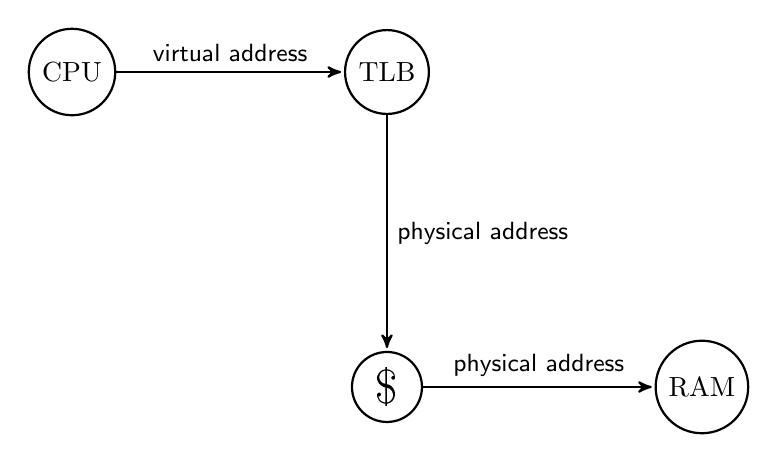
\begin{tikzpicture}[->,>=stealth',shorten >=1pt,auto,node distance=4cm,
	thick,main node/.style={circle,draw}]
	
	\node[main node] (0) {CPU};
	\node[main node] (1) [right of=0] {TLB};
	\node[main node] (2) [below of=1] {\LARGE\$};
	\node[main node] (3) [right of=2] {RAM};
	
	\path[every node/.style={font=\sffamily\small}]
	(0) edge node[] {virtual address} (1)
	(1) edge node[] {physical address} (2)
	(2) edge node[] {physical address} (3);
	\end{tikzpicture}
\end{figure}

\subsubsection{Virtually Addressed Cache}

In a virtually address cache, the CPU accesses cache immediately with the virtual address. On cache-hit, it returns the block of data. On cache-miss, however, the virtual address is sent to the translation look-aside buffer and converted to a physical address. The physical address is then used to access RAM. Since the translation look-aside buffer is not always accessed, virtually addressed caches are faster in the average case. However, there are quite a few issues with a virtually addressed cache. Whenever there is a context switch, the entire cache may need to be flushed --- two processes may use the same virtual address, but their contents are completely different. 

\begin{figure}[H]
	\centering
	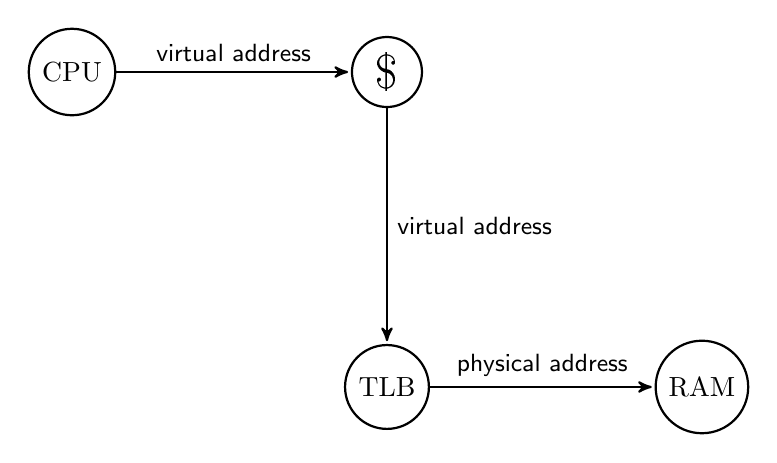
\begin{tikzpicture}[->,>=stealth',shorten >=1pt,auto,node distance=4cm,
	thick,main node/.style={circle,draw}]
	
	\node[main node] (0) {CPU};
	\node[main node] (1) [right of=0] {\LARGE\$};
	\node[main node] (2) [below of=1] {TLB};
	\node[main node] (3) [right of=2] {RAM};
	
	\path[every node/.style={font=\sffamily\small}]
	(0) edge node[] {virtual address} (1)
	(1) edge node[] {virtual address} (2)
	(2) edge node[] {physical address} (3);
	\end{tikzpicture}
\end{figure}

\subsection{Cache Miss Classification}

\subsubsection{Compulsory}

For a compulsory miss, it means that the data was never seen before. A simple example of this is when the CPU first starts and the cache is empty. Any data accessed will have never been seen before.

\subsubsection{Capacity}

For a capacity miss, it means that the cache cannot contain all blocks for which the program requires. Blocks are being swapped in and out constantly.

\subsubsection{Conflict}

For a conflict miss, it pertains to the mapping strategy used. Take for example direct-mapped caches. If all addresses used in the program only accessed one cache line because of the partition bit range, it means that one cache line will be constantly changing while other cache lines are unused.

\subsubsection{Coherence}

Coherence misses come from false sharing due to multi-processors. Suppose there are two processors, each of which has loaded the same block into their cache. Now if one processor updates that block in its own cache, it invalidates the other processor's block. 

\subsection{Fundamental Cache Parameters}

\subsubsection{Cache Size}

Larger caches produces lower miss rates, but also longer access times.

\subsubsection{Block Size}

Small block sizes do not exploit the locality principle and it does not help with compulsory misses.  Larger block sizes, however, may pollute the cache in that it may be grabbing more chunks than necessary. These extra chunks become useless and occupy cache space.

\subsubsection{Associativity}

Larger associativity reduces miss rates, but it becomes slower and harder to build.

\subsubsection{Access Type}

Virtually addressed caches provide lower access times, but on context-switches will require the entire cache to be flushed. Physically addressed caches do not have issues with context switches, but increases it access time as it needs to be go through the translation look-aside buffer each time.

\subsection{Advance Caches}

\begin{itemize}
	\item Small and Simple Cache
	\item Way Prediction Cache
	\item Pseudo Association Cache
	\item Non-Blocking Cache
	\item Multi-Bank Cache
	\item Critical Word First Cache
\end{itemize}

\section{Virtual Memory}

\subsection{Virtual Address Format}

\begin{table}[H]
	\centering
	\begin{tabular}{| c | c |}
		\hline
		Virtual Page Number	&	Offset\\
		\hline
	\end{tabular}
\end{table}

\subsection{Page Table Entry Format}

\begin{table}[H]
	\centering
	\begin{tabular}{| c | c | c |}
		\hline
		Flag Bits	&	Protection Bits	&	Physical Frame Number\\
		\hline
	\end{tabular}
\end{table}

\subsection{Example}

\textbf{Given a 1 Megabyte physical memory, a 30 bit virtual address, and a page size of 8 KB, find the following: number of page frames, bit width of offset, number of entries in the page table and the width of each entry.}

\begin{eqnarray*}
	\text{Number of Page Frames} &=& \text{Size(Physical Memory)} / \text{Size(Page)}\\
		&=& 2^{30} \text{ bytes} / 2^{13} \text{ bytes}\\
		&=& 2^{17} \text{ page frames}
\end{eqnarray*}
\begin{eqnarray*}
	\text{Bit\_Width(Offset)} &=& \text{Number of bits needed to reference 8 KB}\\
	&=& \log_2 2^{13}\\
	&=& 13 \text{ bits}
\end{eqnarray*}
\begin{table}[H]
	\centering
	\caption*{Virtual Address Partition Sizes}
	\begin{tabular}{| c | c | c |}
		\hline
				&	Virtual Page Number	&	Offset\\
		\hline
		Size	&	49 Bits	&	13 Bits\\
		\hline
	\end{tabular}
\end{table}
\begin{eqnarray*}
	\text{Number of Page Table Entries} &=& \text{Number of Virtual Pages}\\
		&=& 2^{\text{Bit\_Width(Virtual Page Number)}}\\
		&=& 2^{49}
\end{eqnarray*}
\begin{eqnarray*}
	\text{Bit\_Width(Page Table Entry)} &=& \text{Number of needed to reference } 2^{17} \text{ page frames}\\
	&=& \log_2 2^{17}\\
	&=& 17 \text{ bits}
\end{eqnarray*}
\section{Multi-Cycle CPU Design}

\section{Pipeline CPU Design}

\end{document}